\DiaryEntry{Game Theory, Mixed-Strategy Equilibrium}{2023-11-24}{Game Theory}

\subsection{Mixed-Strategy Equilibrium}

Some games do not have a Nash equilibrium. Consider, for example, the matching pennies game shown in Figure 9.2. In this game, no strategy profile is stable because each one has a “winner” and a “loser” — a status that is flipped if either player alters his or her strategy. In matching pennies, players actually have an interest in deceiving each other. 

Suppose that player 1 has privately decided to select strategy H. This would be rational if player 1 thought that player 2 would select 2 as well, but player 2's selection of H relies on a belief that player 1 is am likely to play T. In other words, player 1 would like player 2 to believe that player 1 will choose T while, in fact, player 1 plans to select H. Coordination of beliefs and behavior is, in this example, seemingly at odds with best-response behavior.

If one player can accurately predict the other player's strategy, as would be the case in equilibrium, then he can take advantage of the other (for example, by selecting T while he choses H). Therefore, it is not good that other player(s) know which strategy one player is using.

One way to achieve this is to randomize between H and T. This raises the question whether there a mixed-strategy profile that has the equilibrium property?

Note that if each player randomizes with probability $1/2$ on both strategies, then neither player has a strict incentive to play H or T; in fact, all strategies -- H, T, and every mixed strategy -- are best responses to the opponent randomizing with equal probability. To see this, observe that if player 2 plays H and T with equal probabilities, then player 1 will get an expected payoff of zero -- that is, $1/2 \times 1 + 1/2 \times (-1) = 0$ -- regardless of whether player 1 choses H or T. In addition, if player 1 also mixes between H and T, his expected payoff will still be zero.

If we therefore extend the definitions of best response and equilibrium to mixed strategies, we find that the mixed-strategy profile $(1/2, 1/2), (1/2, 1/2)$, where both players randomize equally between their pure strategies, has the Nash equilibrium property in the matching pennies game. With this mixed-strategy profile, each player is best responding to the other. We then can say that the profile $(1/2, 1/2), (1/2, 1/2)$ is a mixed-strategy Nash equilibrium of the matching pennies game.

The formal definition is as follows.

\begin{definition}
    Consider a strategy profile $\sigma = (\sigma_1 , \sigma_2 \ldots, , \sigma_n)$, where $s_i \in \Delta S_i$ for each player $i$. Profile $s$ is a mixed-strategy Nash equilibrium if and only if $u_i(\sigma_i , \sigma_{-i}) \geq u_i(s'_i , \sigma_{-i})$ for each $s'_i \in S_i$ and each player $i$. That is, $\sigma_i$ is a best resposne to $\sigma_{-i}$ for every player $i$.
\end{definition}

For a mixed strategy to be a best response (as required in the definition), it must put positive probability only on pure strategies that are best responses. This demonstrates how to calculate a mixed-strategy Nash equilibrium.

As an example consider the following game which is lobbying game between two firms.

\begin{figure}[H]
    \centering
    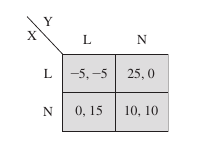
\includegraphics[scale=0.7]{images/2023-11-24-game_theory_01.png}
\end{figure}

Each firm may lobby the government in hopes of persuading the government to make a decision that is favorable to the firm. The two firms, X and Y, independently and simultaneously decide whether to lobby (L) or not (N). Lobbying entails a cost of $15$. Not lobbying costs nothing. If both firms lobby or neither firm lobbies, then the government takes a neutral decision, which yields $10$ to both firms. A firm’s payoff is this value minus the lobbying cost if it lobbied. If firm Y lobbies and firm X does not lobby, then the government makes a decision that favors firm Y, yielding zero to firm X and $30$ to firm Y. Thus, firm Y’s payoff in this case is $30 - 15 = 15$. If firm X lobbies and firm Y does not lobby, then the government makes a decision that favors firm X, yielding $40$ to firm X (so X’s payoff is $40 - 15 = 25$) and zero to firm Y.

There are two pure-strategy Nash equilibria in this game, (N,L) and (L,N); in these points no player has an incentive to deviate from the chosen strategy.

In addition to these pure-strategy equilibria, there is also a mixed-strategy equilibrium. To find it, recall what must hold in a mixed-strategy equilibrium: a player must achieve a best response by selecting a mixed strategy. For example, let’s guess that firm X mixes between L and N. If this strategy is optimal for firm X (in response to the other firm’s strategy), then it must be that the expected payoff from playing L equals the expected payoff from playing N; otherwise, firm X would strictly prefer to pick either L or N.

But how can firm X’s strategies L and N yield the same expected payoff? It must be that firm Y’s behavior generates this expectation (because if firm Y played a pure strategy, then X would strictly prefer one of its strategies over the other). Let $q$ denote the probability that firm Y plays L; that is, $(q, 1 - q)$ is firm Y’s mixed strategy. Against this mixed strategy, firm X expects to earn

\bee
q(-5) + (1-q)25 = 25 - 30q
\eee

by choosing L and

\bee
q0 + (1-q)10 = 10 - 10q
\eee

by choosing N. For firm X to be willing to randomize, it must be that $25 - 30q = 10 - 10q$. This simplifies to $q = 3/4$. In other words, firm X can randomize in playing a best response if firm Y’s strategy is $(3/4, 1/4)$.

Let us move on to firm Y’s incentives and let $p$ be the probability that firm X plays L. Then, if firm Y selects L, its expected payoff is

\bee
p(-5) + (1-p)15 = 15 - 20p
\eee

By choosing N, its expected payoff is

\bee
p0 + (1-p)10 = 10-10p
\eee

Firm Y is indifferent between its two strategies (and therefore willing to randomize) if $15 - 20p = 10 - 10p$, which simplifies to $p = 1/2$.

The mixed-strategy profile $((1/2, 1/2), (3/4, 1/4))$ is a mixed-strategy Nash equilibrium. Given firm Y’s mixed strategy, firm X’s mixed strategy is a best response -- in fact, every strategy is a best response for firm X. Likewise, given firm X’s strategy, firm Y’s prescribed strategy is a best response. Note that constructing a mixed-strategy equilibrium entails an interesting new twist: we look for a mixed strategy for one player that makes the other player indifferent between her pure strategies. This is the best method of calculating mixed-strategy equilibria.

\subsection{Strictly Competitive Games}

We next consider \emph{strictly competitive games}. Here, the two players have exactly opposite rankings over the outcomes. Wherever one player’s payoff increases, the other player’s payoff decreases. Strictly competitive games offer no room for joint gain or compromise.

\begin{definition}
A two-player, strictly competitive game is a two-player game with the property that for every two strategy profiles $s, s' \in S$, $u_1(s) > u_1(s')$ iff $u_2(s) < u_2(s')$.
\end{definition}

Matching pennies is a good example of a two-player, strictly competitive game. There are only two payoff vectors in matching pennies, one that favors player 1 and one that favors player 2. The payoff vectors describe
who wins the game.

Lots of games have outcomes that are limited to: (a) player 1 wins and player 2 loses, (b) player 2 wins and player 1
loses, and (c) the players tie (draw). Because players prefer winning to tying and tying to losing, every two-player game with outcomes described in this way is a strictly competitive game. Such games include chess, checkers, tennis, etc. These games are additionally all \emph{zero-sum} games in which the players’ payoffs always sum to zero.

Note that there are strictly competitive games which are not zero-sum. As an example, consider the game in the following Figure.

\begin{figure}[H]
    \centering
    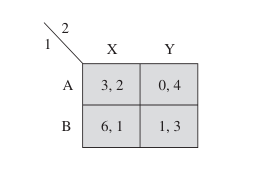
\includegraphics[scale=0.7]{images/2023-11-24-game_theory_02.png}
\end{figure}

\subsection{Security Strategies}

We next consider the worst-case scenario for every player in a game. In any game, the worst payoff that player $i$ can get when he plays strategy $s_i$ is defined by

\bee
w_i(s_i) = \min_{s_j \in S_j} u_i(s_i, s_j)
\eee

We look at player $j$'s strategies to find the one that gives player $i$ the lowest payoff given that player $i$ plays strategy $s_i$. If player $i$ plays strategy $s_i$, then he will get \emph{at least} the payoff $w_i(s_i)$. 

In the game shown in the previous subsection, if player $1$ plays strategy A, he gets the worst payoff (of $0$) when player $2$ plays strategy Y.

We can now search for a strategy which maximizes the worst payoff. Such a strategy is called a \emph{security strategy} is defined as follows.

\begin{definition}
A strategy $\underline{s}_i \in S_i$ for player $i$ is called a security strategy if

\bee
\underline{s}_i = \arg \max_{s_i \in S_i} w_i(s_i)
\eee

Player $i$'s security payoff level is is defined as

\bee
\max_{s_i \in S_i} w_i(s_i) = \max_{s_i \in S_i} \min_{s_j \in S_j} u_i(s_i, s_j)
\eee
\end{definition}

In the game shown in the previous subsection, strategy B is player $1$'s security strategy as it maximizes the worst payoff (which is reached when player $2$ plays strategy Y); the security payoff level of player $1$ is therefore $1$.

In a similar spirit, Y is player $2$'s security strategy and the security payoff level of player $2$ is $3$.

Above definitions were done for pure strategies; we can extend all concepts to mixed strategies as well. In this case we call a strategy which maximizes the \emph{expected} worst-payoff a \emph{max-min strategy} and it realizes an \emph{expected max-min payoff level}. However, one realisation of a game using the max-min strategy may yield a worse payoff than the expected value.

There is a connection between max-min strategies and Nash equilibria for two-player strictly competitive games.

\begin{theorem}
If a two-player game is strictly competitive and has a Nash equilibrium $s^\star \in S$, then $s^\star_1$ is a security strategy for player 1 and $s^\star_2$ is a security strategy for player 2. Furthermore, each player’s security level and maxmin level are the same, so $s^\star_1$ and $s^\star_2$ are maxmin strategies for the players as well.	
\end{theorem}

In other words, if $s_i$ is a Nash-equilibrium strategy for player i in a strictly competitive game, then $s_i$ guarantees player i at least her security payoff level, and player i cannot improve this lower bound by randomizing. In our example, (B, Y) is a Nash equilibrium of the game, and above we observed that B and Y are security strategies.



%%% Local Variables:
%%% mode: latex
%%% TeX-master: "journal"
%%% End:
